\documentclass[12pt, preprint]{aastex}
\usepackage{float}
\doublespace
\begin{document}

\title{Physics 785 Term Paper: Turbulence in Molecular Clouds: Origins \&
Impacts}
\author{Ben Keller}
\maketitle
\newpage
\section{Introduction}
The phenomenon of turbulence is one of the most heavily studied, and yet poorly
understood processes in astrophysics.  It can influence the flow of fluids across
length scales spanning more than a dozen orders of magnitude, and can affect
astrophysical processes at every scale, from dense cores \citep{larson1981} up to the intergalactic
medium (\citet{scan2013} suggests that galactic outflows can be
driven by the decay of turbulence in the ISM).  In this paper, I will review 
the current understanding of turbulence in the context of molecular clouds.  I
will focus primarily on how turbulence can arise within a cloud (primarily in terms of
energy balance), and how it can drive the evolution of that cloud by promoting
or preventing cloud coalescence, dispersal, and star formation within clouds.

Molecular clouds are important locations for ISM chemistry and physics.  Though
they occupy only $0.05\%$ of the ISM by volume, they contain roughly $20\%$ of
the mass of the ISM.  The high densities ($>300 cm^{-3}$) and low temperatures
($<100K$) make them important sites for ISM chemistry, and the location of most of
the clustered and massive star formation within galaxies\citep{tiel2010}

\section{Basic Turbulence Theory}
\subsection{Kolmogorov's 1941 Theory}
Nearly all modern theories of turbulence are build upon the Kolmogorov's 1941
theory \citep{kolm1991}.  The Kolmogorov theory of turbulence describes locally
homogeneous, locally isotropic turbulence (a reasonable assumption for turbulent
flow with large Reynolds numbers, which certainly holds in all the phases of the
ISM).  Kolmogorov proposed two key hypotheses. The first is that the distribution 
of velocities in a turbulent flow are uniquely determined by the viscosity 
$\nu$ and the average specific dispersion energy rate $\epsilon$,  From 
this, a characteristic length $\eta$ and velocity $\sigma$:
$$\eta = \nu^{3/4}\epsilon^{1/4}$$
$$\sigma = \sqrt{\nu/\epsilon}$$
The second hypothesis is that on scales much larger than $\eta$, the turbulent flow
is uniquely determined \textit{only} by $\epsilon$.  These two assumptions
allow you to uniquely determine a energy spectrum as a function of wavenumber
$k$:
$$E(k) \propto \epsilon^{2/3}k^{-5/3}$$
The Kolmogorov energy spectrum has been the foundation of nearly all subsequent
theories of turbulence.  The negative power law slope can be seen as the cascade
of energy down from large scale turbulent motions down to scales where viscous
dissipation becomes important ($\lambda \approx \eta$).
\subsection{MHD Turbulence}
Modern theories of turbulence in molecular clouds rely on the interplay between
``pure" fluid turbulence, and turbulence within magnetic fields.  By storing
energy within these fields, the decay of turbulence can be delayed long enough
to allow more modest energy sources to drive the turbulence observed in
molecular clouds.  \citet{shu1987} reports magnetic field strengths in a number
of molecular clouds on the order of $10-100 \mu G$.  Simple virial/equipartition
arguments suggest that thermal, turbulent, and magnetic energies within a cloud
should be roughly equal.

The biggest difference between hydrodynamic and MHD turbulence is the breaking
of Kolmogorov's assumption of isotropy.  The presence of magnetic field lines
impose a preferred direction for the fluid flow (namely along these field
lines).  This anisotropy can produce density gradients perpendicular to field
lines.  In addition to these changes, magnetised fluids can also transport MHD
waves, namely shear and compression Alfv\'{e}n waves (travelling along vs.
across field lines respectively).  Since these oscillations have a different
characteristic speed than the acoustic waves of Kolmogorov turbulence, they can
result in a different power spectrum for turbulent modes, and their anisotropy
means that wavenumbers parallel to field lines $k_\parallel$ have a different
energy contribution to those perpendicular to the field $k_\perp$.  However, a
mixing of these two modes can allow for a average power spectrum to be derived
that approaches the values seen in isotropic MHD turbulence.  For
isotropic MHD turbulence, the power spectrum derived by \citet{irosh1964} is a
similar power-law spectrum to the Kolmogorov, with a $-3/2$ slope.  In the
strong-field limit, this approximation matches reasonable with simulated and
theoretical results.  In weak and intermediate fields, however, local conditions
can have a significant effect on the energy spectrum.  

MHD also provides new modes for turbulent energy to decay.  Ohmic heating and
ambipolar diffusion can convert turbulent energy within the fluid directly into
heat, and dynamo processes can pull kinetic energy out of the fluid and store it
in magnetic fields.  3D simulations of MHD turbulence suggest it decays in
approximately $\tau_{cross} = L/v_{rms}$, where $L$ is the scale of the cloud,
and $v_{rms}$ is the rms turbulent velocity. In environments like molecular
clouds, where turbulence is highly supersonic, the effects of MHD vs. ``pure"
hydrodynamic turbulence may be small \citep{elm2004}

\section{Observational Evidence}
Direct observations of turbulence have been made by looking at the velocity
spectrum in molecular hydrogen tracer elements (commonly $^{12}CO$ and
$^{13}CO$). The velocity dispersion $\sigma$ in a region of size $L$ can be
derived from the Kolmogorov power spectrum, and is found to be:
$$\sigma \propto L^{1/3}$$
for the $-5/3$ power-law energy spectrum \citep{larson1979}.
\citet{larson1979} used observations of $CO$ and $HI$ within cool
clouds, along with the velocity dispersion of stellar spectra collected from
young (less than a few $Gyr$ old) stars to estimate the dispersion in cool clouds.  
The use of young stars was justified by the fact that they should retain the
momentum of the gas they formed from.  His
observation covered scales from a few $pc$ up to $20 kpc$.  Figure 1 shows
the relationship he found between region size and the velocity dispersion
within these regions is in good agreement with the $1/3$ slope power law
predicted by Kolmogorov turbulence.
More recent works have used additional statistical and numerical tools to detect
turbulence.  \citet{brunt2003} used principal component analysis of $^{12}CO$
emission in the FCRAO radio telescope's Outer Galaxy Survey.  to calculate the
power spectrum of molecular clouds in the outer galaxy.  He found values for the
power spectrum slope $\beta$ ranging $\approx 1.5$ to $\approx 3$, bounding the
Kolmogorov value of $5/3$.

\begin{figure}[H]
	\centering
	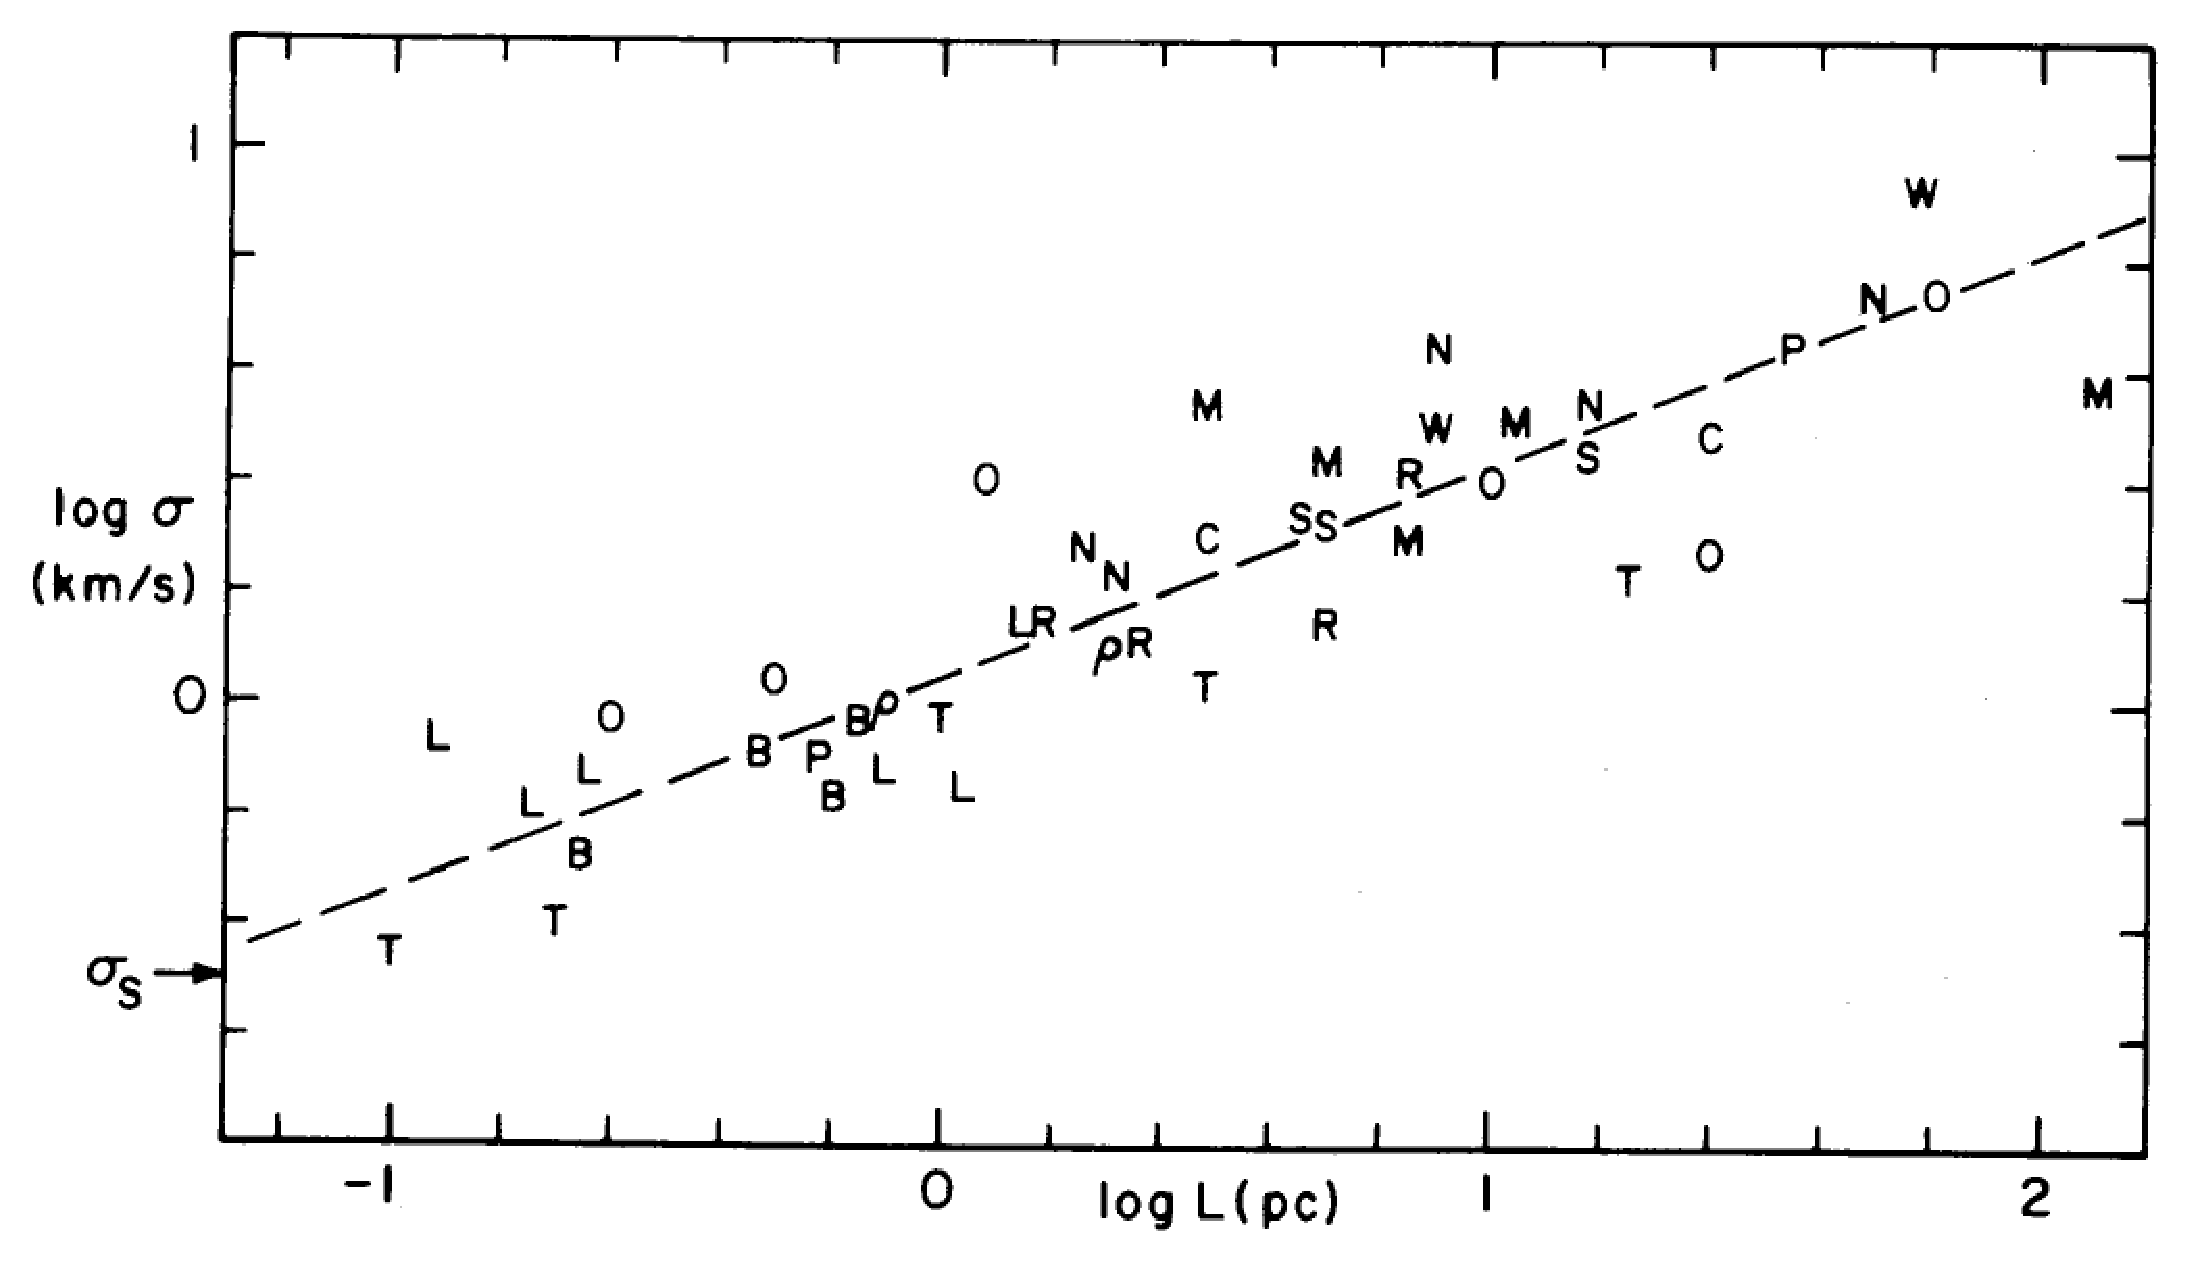
\includegraphics[scale=0.4]{figures/larsonlaw_larson1981.eps}
	\caption{\citet{larson1981}'s results showing a tight correlation between
	the velocity dispersion within a cloud and the size scale of that cloud.
The slope of the fitted line is 0.38, while the slope of the Kolmogorov
density-velocity dispersion PDF is 1/3.}
\end{figure}
\section{Origins of Turbulence}
The observation of turbulence in molecular clouds raises two major questions.
Firstly, from whence does the energy within the turbulent motions come, and
secondly, how does this energy convert from whatever form it arrives in into 
turbulent motion.

Unlike turbulence on larger scales, which can be driven by galactic rotations
and motions of clouds through the galactic ISM \citep{balb1991}, turbulence in
molecular clouds is primarily powered by local sources of energy.  Since
turbulence is rapidly dissipated, a constant input of energy is needed to keep
it from simply decaying down the Kolmogorov microscales and converting into
heat.  This decay is characterised by the rms Mach number $M_{rms}$, the Jeans
length $\lambda_J$, free-fall time $\tau_{ff}$ and the characteristic driving 
wavelength of the turbulence $\lambda_T$ \citep{mac1999}:
$$ \tau_D \approx 3.9 \frac{\tau_{ff}\lambda_D}{M_{rms}\lambda_J}$$
The values of $\lambda_D$ and $\lambda_J$ for molecular clouds is not
well-known, but the ratio of the two is expected to be on the order of 1-10
\citep{mac2004}.

Once a molecular cloud has begun forming stars, stellar feedback can provide
ample energy to drive both bulk and turbulent motions within clouds.
\citet{agertz2012} reports that stars typically return 
$\approx 10^{34} erg s^{1-} M_\odot^{-1}$ in the form of stellar winds and
supernovae.  Massive stars also produce ionising UV, generating HII regions that
can shock the surrounding molecular gas.  With even conservative estimates of
efficiencies between the feedback rates, stellar feedback combined with
turbulence generated by fluid instabilities in the formation of molecular clouds
provides sufficient energy to power the observed turbulence within molecular
clouds\citep{elm2004}.  The chaotic driving of supernovae blasts and wind-carved
bubbles on a scale of $50-500pc$ (ie, on the scales comparable tot the total
cloud size), which then cascades down the to smaller scales.
\section{Impact of Turbulence on Cloud Structure \& Evolution}
\subsection{Cloud Formation}
The largest effect of turbulence on molecular clouds may not be intra-cloud
phenomena, but instead the actual \textit{formation} of clouds.
\citet{larson1981} suggested from his observations that cloud lifetimes were on
the order of $10^7 yr$, about twice their free-fall time.  If most clouds are
this young, this implies that clouds are both formed and destroyed on a
relatively continuous and rapid basis. Recent simulation results from
\citet{hopk2011} support this picture of a constantly replenished supply of
short-lived GMCs, and some suggest that even shorter lifetimes of a few $10^6$
years are more likely \cite{mac2004}.

Early models of cloud formation relied on a hierarchical merger type picture of
cloud collision and coalescence to explain the production of giant molecular
clouds from the atomic and ionised medium.  \citet{larson1981} reports that
these models fail to produce the production rates needed to sustain the observed
abundance of molecular clouds in the galaxy in light of their relatively short
lifetime (these models were developed with the assumption that cloud lifetimes
were on the order of $10^8 yr$).  Turbulence within the larger ISM can produce, 
in the highly compressible supersonic regime observed, strong density perturbations and
clumpy, filamentary structures like that seen in figure 2.  \citet{val2006}
presents a picture of supersonic turbulence or colliding flows producing thin, 
shocked sheets that then fragments to form molecular clouds. Coupled with
thermal multiphase instabilities, this can act to rapidly build dense clumps
that will quickly become molecular clouds as atomic hydrogen becomes molecular
on dust grains and the high densities of the cloud allow for self-shielding.
The dominant theory of cloud formation currently is that shocks, from turbulence
and supernovae, build large overdensities where molecule formation is very
rapid, and that cloud dispersal by feedback (or the same turbulent flow that
can form them) happens on the order of a roughly 1-10 Myr.

\begin{figure}[H]
	\centering
	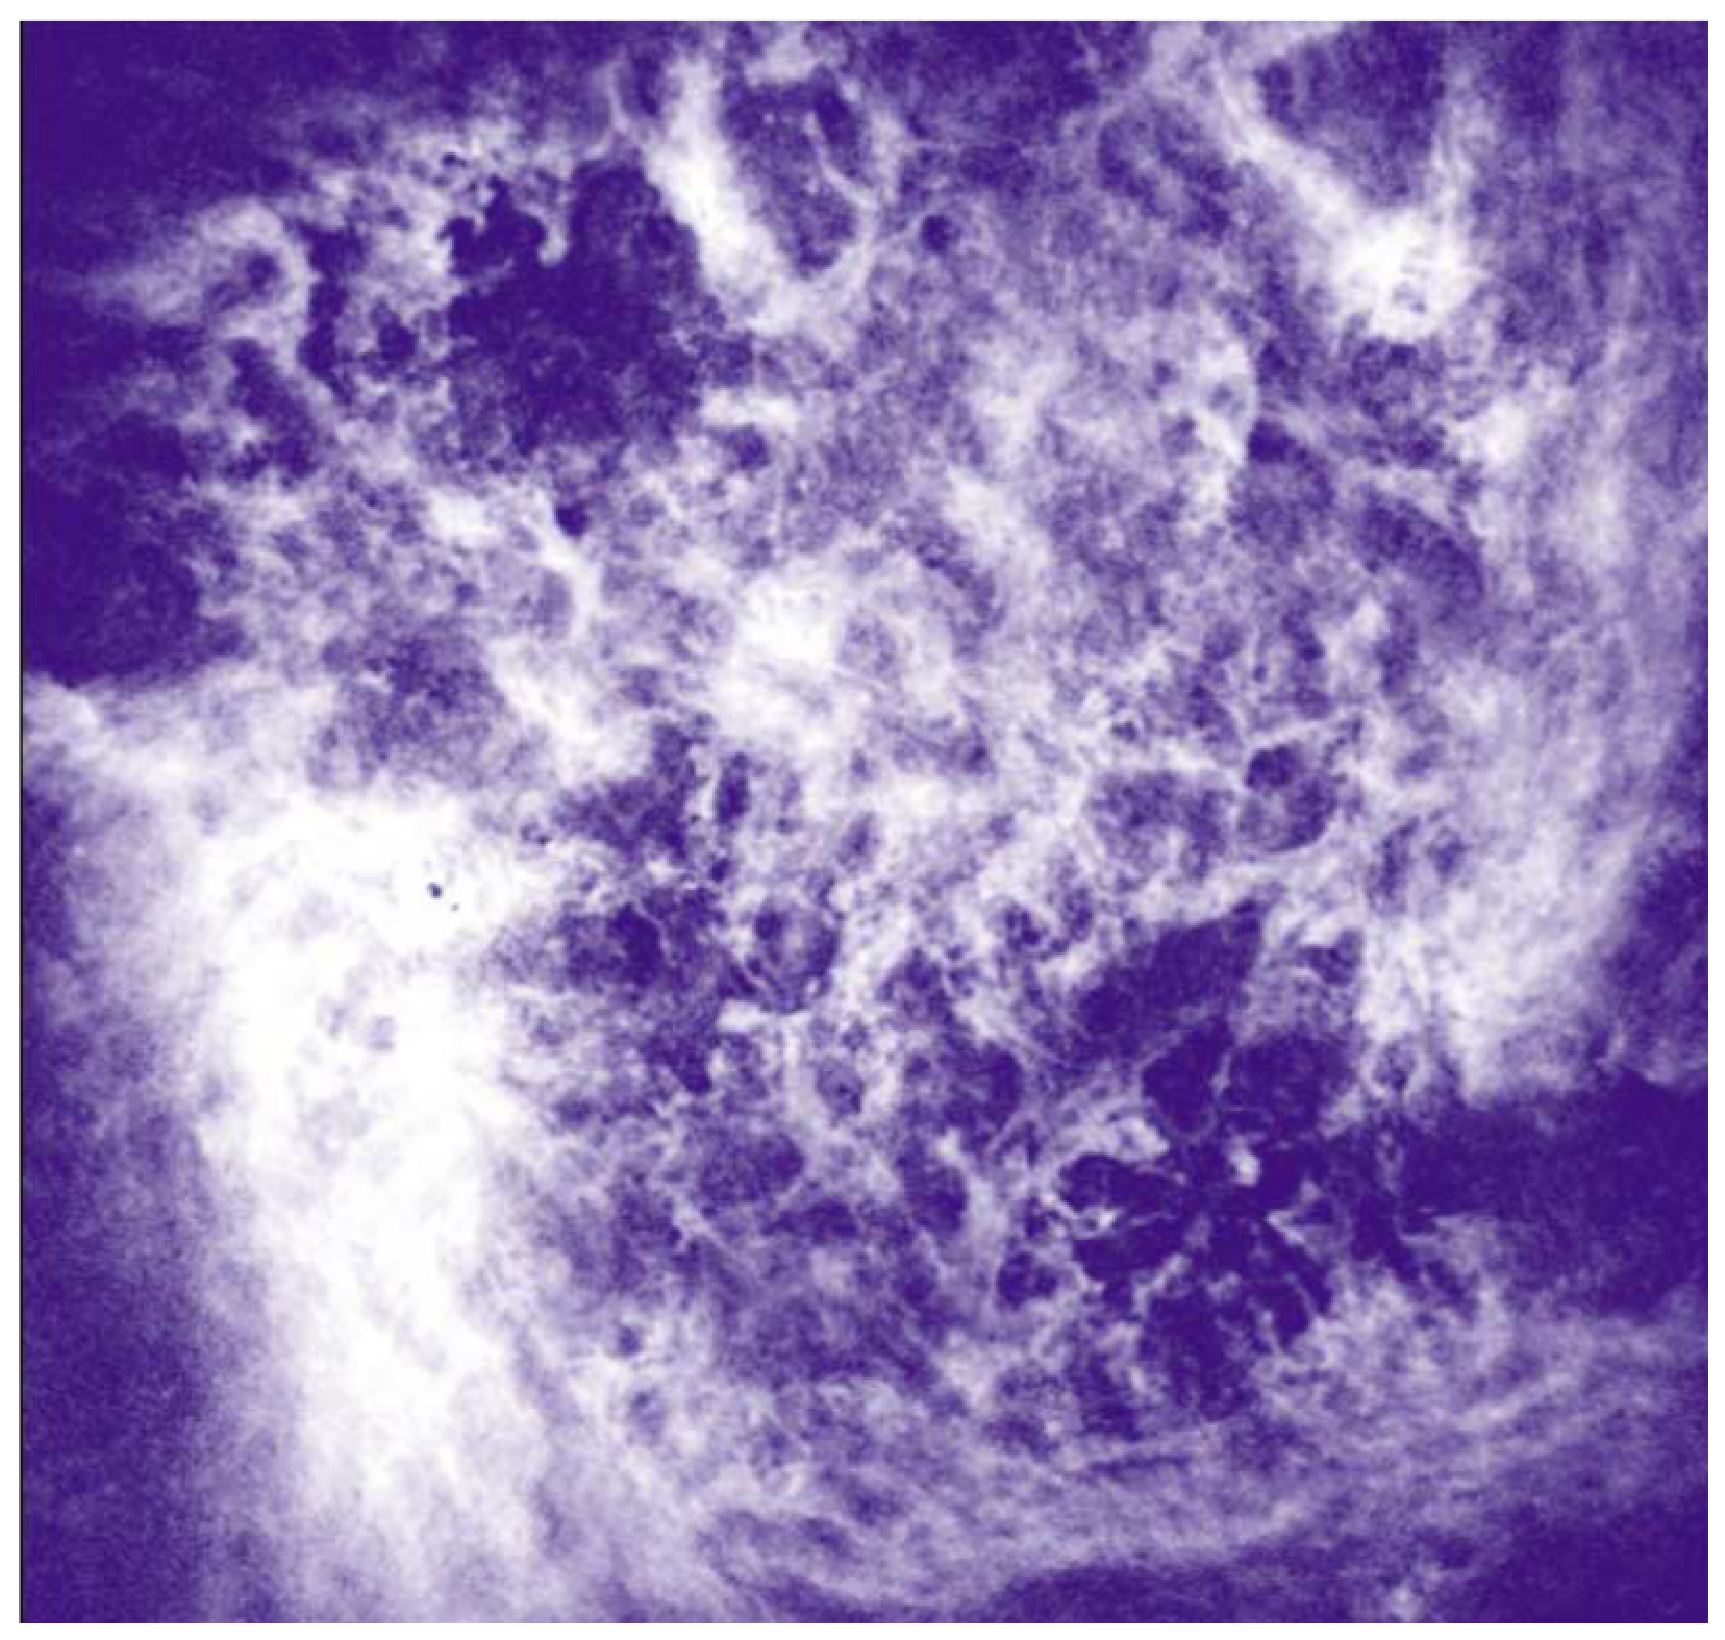
\includegraphics[scale=0.4]{figures/turbulent_LMC_elm2004.eps}
	\caption{21cm emission from the Large Magellanic Cloud.  Note the
		filiaments, voids, and clumps in this HI emission map.  These
		structures, and the associated 2D power spectrum of them, are closely
		associated with turbulent motions, and can lead to the rapid production
	of molecular clouds in overdense regions.  Image from \citet{elm2004}.}
\end{figure}
\subsection{Turbulent Pressure Support}
Observations of molecular clouds provide two perplexing facts, namely that they
are typically cold (10-100K), and massive (much larger than the Jeans mass
$M_J$) \citep{gold1978}.  This, coupled with their relatively short lifetimes,
seems to imply that they collapse gravitationally relatively quickly after they 
form.  However, measurements of star formation efficiency within these clouds,
and of the relative stellar mass fractions of the milky way and other galaxies
tells us that these clouds only convert a small fraction of their mass into
stars \citep{mac2004}, and that their lifetimes are in fact longer than their
free-fall times. This suggests that
a there is some sort of non-thermal pressure supporting these clouds, in
addition to processes that can disrupt or destroy clouds before they can convert
most of their mass into stars. While disruption of clouds by feedback can reduce
their star formation efficiency (by destroying them after they form only a few
massive stars)\citep{hopk2011}, the observation of super-Jeans mass clouds that
are older than the time needed for them to collapse needs this additional
mechanism to keep clouds supported.
In molecular clouds that are in hydrostatic equilibrium, determining the sources
of pressure that supports the clouds against gravitational collapse is key in
determining which clouds will collapse, and why.  Non-thermal pressure support is
essential to allow super-Jeans mass clouds to persist.

Treating the energy within a volume's turbulence as  a source of pressure was
proposed as early as \citet{chandra1951}, where the Jeans stability criteria is
modified from:
$$\lambda_J = 2\pi \sqrt{\frac{c_s^2}{4\pi G\rho}}$$
where $c_s$ is the sound speed, to a smaller value derived using the mean
turbulent velocity $u$:
$$\lambda_J = 2\pi \sqrt{\frac{c_s^2+u^2/3}{4\pi G\rho}}$$
For molecular clouds, where turbulence tends to be highly supersonic, this can
act to significantly increase the stability of a cloud against gravitational
collapse.
\subsection{Mixing \& Chemistry}
Molecular clouds, being \textit{molecular}, are sites in which more 
complicated ISM chemistry can occur.  Since these clouds are extremely dense and
cool, while many of the reactants for forming simple ($CO$, $HCN$, etc.) and
complex (PAHs, amino acids, etc) are abundant, the conditions in the molecular
cloud are often not ideal for slow, steady formation of these compounds.
PDRs at the edge of clouds can catalyse the formation of some compounds, but
destroy others.  Many of the compounds in molecular clouds have negative heats
of formation, implying they would form extremely slowly at the mean $\approx
10K$ temperatures in the cloud.  In addition to this, chemical reaction networks
found that early-time solutions to time-dependent evolution equations (rather
than equilibrium concentrations) matched most closely the observed abundances in
molecular clouds\citep{scalo2004}.

Turbulence offers an explanation for all of these observations.  Since the
interiors of clouds are not homogeneous in density, temperature, or UV flux,
turbulent mixing can transport species into regions where their production is
enhanced, and then spread the products into the rest of the cloud.  Decay of
turbulence and shock heating can result in local temperature increases, allowing 
endothermic reactions to produce species that otherwise would not be 
seen\citep{xie1995}.  MHD turbulence
can have a significant impact on ion-neutral reactions by magnetically forcing
ions, producing an effectively faster mixing rate for ionised species.
\subsection{Larson's Laws \& Star formation}
Strangely, turbulence can both support clouds (on a global scale), and cause
collapse (on smaller scales) \citep{mac2004}.  Since molecular cloud
turbulence is often supersonic, it is well beyond the incompressible regime,
and can produce density perturbations that can then collapse to form
stars\citep{elm2004}. Turbulence in nascent star forming 
regions is a critical element in the modern theory 
of star formation. One of the earliest works proposing this connection is
\citet{larson1981}.  Building on previous "merging bubble/shell" models of
molecular clouds and the larger ISM from works such as \citet{norman1980} and
\citet{mckee1977}, Larson used $^{13}CO$ observations of Taurus, $\rho$
Ophiucus, Orion, and a number of other clouds to determine a the mass function
of clouds within these clumps.  By measuring the velocity dispersions of these
clouds, along with their dimension, he observed that $\sigma \propto L^{0.38}$
(the ``size-linewidth" relation).  Since this value is close to the Kolmogorov
real-space power law slope $1/3$, \citet{larson1981} argued that the size of
clumps within molecular clouds was determined primarily by turbulence within
the cloud.

One of the most interesting recent developments is the suggestion by
\citet{hopk2013} that the
shape and universality of the stellar initial mass function is the result of 
turbulent dynamics within
star forming clouds. \citet{hopk2013} proposes a model of gravo-turbulent
fragmentation using the excursion set formalism similar to that previously used 
successfully to predict the Halo Mass Function and clustering rates in
large-scale cosmological structures by \citet{press1974}.  By applying this tool
to the turbulent fluid of a molecular cloud, and tracking the first and last
crossings of overdense perturbations (see figures 3 and 4), the mass function of
protostellar cores, (and thus the IMF) can be predicted using Monte Carlo
realisations of the turbulent density spectrum.  This analytic framework
can be used to generally predict the mass function from fragmentation
on any scale from essentially first principles (including the formation 
of clouds themselves, if they do in fact
form from turbulent fragmentation).  This framework suggests that gravitational
collapse of turbulent overdensity is the dominant driving force for much of the
substructure within molecular clouds.

\begin{figure}[H] 
	\centering
	\includegraphics[scale=0.3]{figures/structure_hopk2013.eps}
	\caption{The key feature of \citet{hopk2013}'s theory of turbulent
		fragmentation is the transition across the line of stability (dashed
		red) where overdensities can collapse.  This line shows when
		gravitational potential overwhelms internal support.  By evalauating realizations of turbulent
		overdensities, the spectrum of overdensities that cross this barrier and
	become bound can be determined.}
\end{figure}

\begin{figure}[H] 
	\centering
	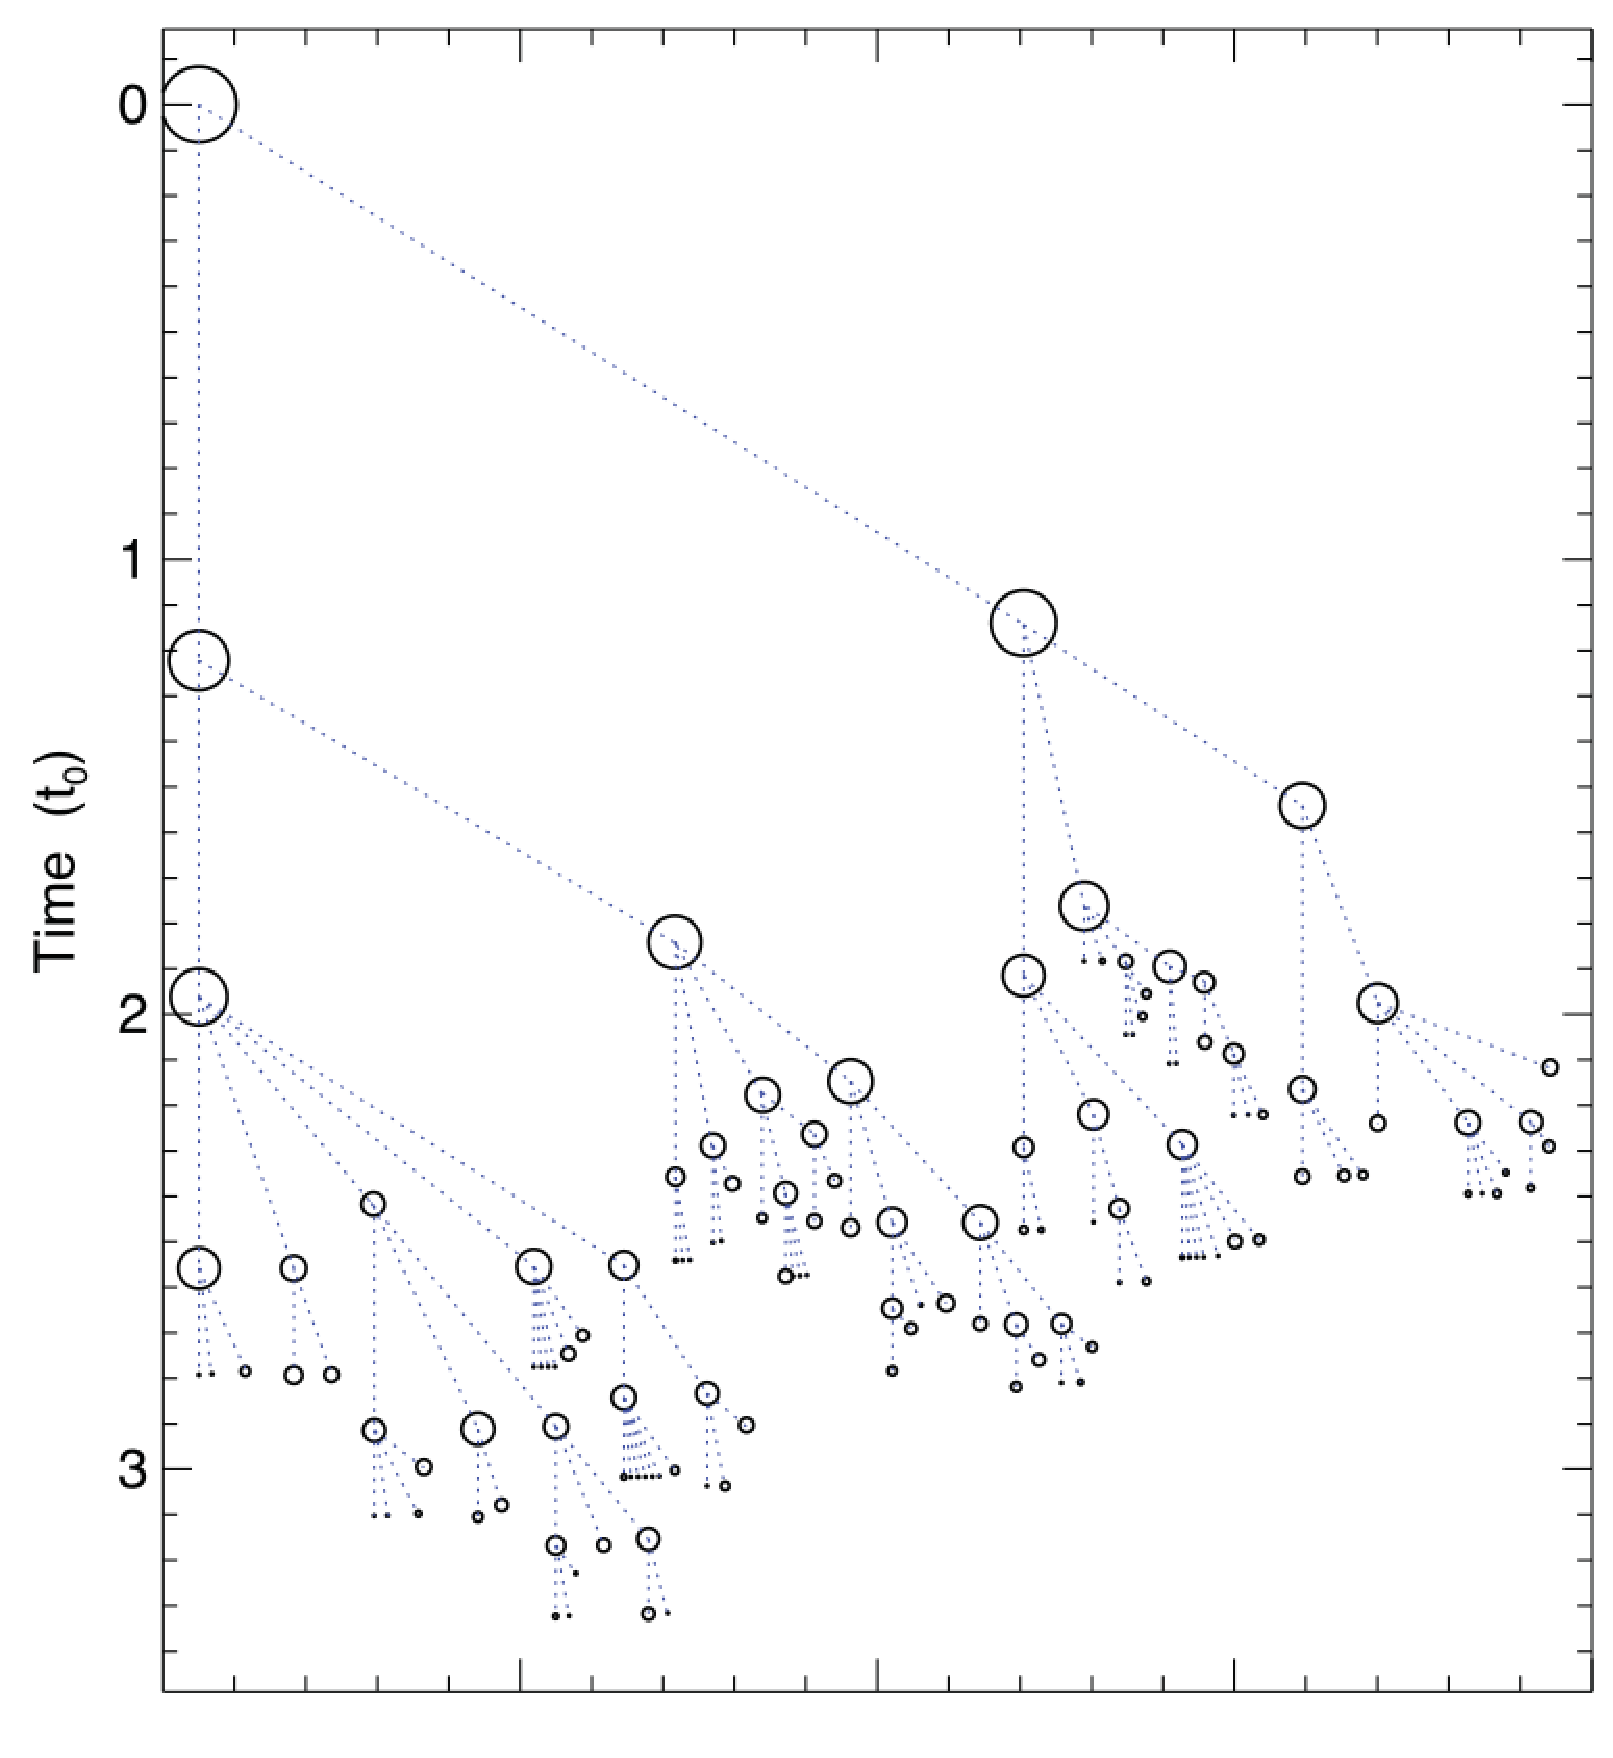
\includegraphics[scale=0.3]{figures/fragtree_hopk2013.eps}
	\caption{In the \citet{hopk2013} model, turbulent overdensities fragment
	over time in a cascading ``tree", producing a spectrum of clump/cloud sizes}
\end{figure}

\section{Conclusion}
It is clear that on every scale related to the physics of molecular clouds, from
the atomic and molecular chemical processes within them, to the actual formation
of the clouds themselves, turbulence is a key ingredient.  Theoretical
predictions from as early as 1951, and observations from the 1970s confirmed
that turbulence was deeply related to the internal structure and evolution of
molecular clouds.  Recent work has continued to build upon this, suggesting that
the chemistry of the molecular ISM, and the mass function of stars are also 
closely tied to the turbulent motions within molecular clouds.  As simulations
and observations further constrain the energy spectrum, growth rate, and
dissipation of turbulence, a key component to building a unified picture 
of molecular cloud creation and destruction, star formation, and interstellar 
chemistry will be complete.

\begin{thebibliography}{}
	\bibitem[Chandrasekhar(1951)]{chandra1951} Chandrasekhar, S.\ 1951, 
		Royal Society of London Proceedings Series A, 210, 26 
	\bibitem[Iroshnikov(1964)]{irosh1964} Iroshnikov, P.~S.\ 1964, 
		\sovast, 7, 566 
	\bibitem[Press \& Schechter(1974)]{press1974} Press, W.~H., \& Schechter, P.\
			1974, \apj, 187, 425 
	\bibitem[McKee \& Ostriker(1977)]{mckee1977} McKee, C.~F., \& Ostriker,
			J.~P.\ 1977, \apj, 218, 148 
	\bibitem[Goldsmith \& Langer(1978)]{gold1978} Goldsmith, P.~F., \& Langer,
			W.~D.\ 1978, \apj, 222, 881 
	\bibitem[Larson(1979)]{larson1979} Larson, R.~B.\ 1979, \mnras, 
		186, 479 
	\bibitem[Norman \& Silk(1980)]{norman1980} Norman, C., \& Silk, J.\ 
		1980, \apj,	238, 158 
	\bibitem[Larson(1981)]{larson1981} Larson, R.~B.\ 1981, \mnras, 
		194, 809 
	\bibitem[Shu, Adams \& Lizano(1987)]{shu1987} Shu, F. H., Adams, F.C.,
		Lizano, S.\ 1987 \araa, 25, 23
	\bibitem[Balbus \& Hawley(1991)]{balb1991} Balbus, S.~A., \& Hawley, J.~F.\
			1991, \apj, 376, 214 
	\bibitem[Kolmogorov(1991)]{kolm1991} Kolmogorov, A.~N.\ 1991, 
		Royal Society of London Proceedings Series A, 434, 9 
	\bibitem[Xie et al.(1995)]{xie1995} Xie, T., Allen, M., 
		\& Langer, W.~D.\ 1995, \apj, 440, 674 
	\bibitem[Evans (1999)]{evans1999} Evans, N. J.\
			1999, \araa, 37, 311
	\bibitem[Mac Low(1999)]{mac1999} Mac Low, M.-M.\ 1999, \apj, 
		524, 169 
	\bibitem[Brunt(2003)]{brunt2003} Brunt, C.~M.\ 2003, \apj, 583, 
		280 
	\bibitem[Elmegreen \& Scalo(2004)]{elm2004} Elmegreen, B.~G., \& Scalo, J.\
			2004, \araa, 42, 211 
	\bibitem[Scalo 	\& Elmegreen(2004)]{scalo2004} Scalo, J., \& Elmegreen, B.~G.\
			2004, \araa, 42, 275
	\bibitem[Mac Low \& Klessen(2004)]{mac2004} Mac Low, M.-M., \& Klessen,
		R.~S.\ 2004, Reviews of Modern Physics, 76, 125 
	\bibitem[V{\'a}zquez-Semadeni et al.(2006)]{val2006}
		V{\'a}zquez-Semadeni, E., Ryu, D., Passot, T., Gonz{\'a}lez, R.~F., 
		\& Gazol, A.\ 2006, \apj, 643, 245 
	\bibitem[Tielens(2010)]{tiel2010} Tielens, A.~G.~G.~M.\ 2010, 
		The Physics and Chemistry of the Interstellar Medium, by 
		A.~G.~G.~M.~Tielens, Cambridge, UK: Cambridge University Press,	2010
	\bibitem[Hopkins et al.(2011)]{hopk2011} Hopkins, P.~F., 
		Quataert, E., \& Murray, N.\ 2011, \mnras, 417, 950 
	\bibitem[Crutcher(2012)]{crutch2012} Crutcher, R.~M.\ 2012, \araa,
		50, 29 
	\bibitem[Agertz et al.(2012)]{agertz2012} Agertz, O., Kravtsov, 
		A.~V., Leitner, S.~N., \& Gnedin, N.~Y.\ 2012, arXiv:1210.4957 
	\bibitem[Hopkins(2013)]{hopk2013} Hopkins, P.~F.\ 2013, \mnras, 
		729 
	\bibitem[Scannapieco(2013)]{scan2013} Scannapieco, E.\ 2013, \apjl, 763, L31 
\end{thebibliography}




\end{document}
